\begin{frame}

    \frametitle{Schéma}

    Moyennant une stratégie de scission (splitting), le schéma
    numérique s'exprime comme une combinaison de l'integration du
    processus d'Ornstein-Uhlenbeck et le schéma de Verlet :
    %
    \begin{align*}
        \tilde p_1^n &= \alpha p_1^n + \sigma_L G_1^n, \\
        \tilde p_N^n &= F + \alpha (p_N^n - F) + \sigma_R G_N^n, \\
        \tilde p_i^n &= p_i^n, i \neq 1,N, \\
        %
        p_i^{n+1/2} &= \tilde p_i^n - \frac{\Delta t}{2}
        \frac{H}{q_i} (q^n, \tilde p^n), \\
        %
        q_i^{n+1} &= q_i^n+ \Delta t p_i^{n+1/2}, \\
        %
        p_i^{n+1} &= p_i^{n+1/2} i - \frac{\Delta t}{2}
        \frac{H}{q_i} (q^{n+1}, p^{n+1/2}),
    \end{align*}
    %
    où $\alpha = e^{-\gamma \Delta t}$,
    $\sigma_L = \sqrt{(1 - \alpha^2)T_L}$,
    et $\sigma_R = \sqrt{(1 - \alpha^2)T_R}$.
    Et $G_1^n$ et $G_1^N$ sont des variables aléatoires gaussiennes.

\end{frame}

\begin{frame}

    \frametitle{Schéma}

    Les 3 premières lignes du schéma constituent l'intégration
    du processus d'Ornstein-Uhlenbeck, qui représente l'influence
    des thermostats et du forçage sur le système. Les thermostats
    n'agissent que sur le premier et le dernier rotor ($i = 1,N$).

    Les 3 dernières lignes constituent le schéma de Verlet, qui
    représente l'évolution Hamiltonienne du système.

    Pour toutes les expériences numériques $\gamma = 1$, et on
    utilise un pas de temps $\Delta t = 0.05$.

\end{frame}





\begin{frame}

    \frametitle{Schéma d'Ornstein-Uhlenbeck}

    Dans les équations d'évolution il y a une partie liée à l'Hamiltonien,
    et une partie stochastique (pour les rotors à gauche et à droite).

    La partie stochastique est le processus d'Ornstein-Uhlenbeck, qui
    s'écrit
    %
    \[dp_t = \theta (\mu - p_t) dt + \sigma dW_t\]
    %
    Pour le rotor à gauche, on a
    $\theta = \gamma$, $\mu = 0$, et $\sigma = \sqrt{2 \gamma T_L}$.
    Pour le rotor à droite, on a
    $\theta = \gamma$, $\mu = F / \gamma$, et $\sigma = \sqrt{2 \gamma T_R}$.

\end{frame}






\begin{frame}

    \frametitle{Schéma d'Ornstein-Uhlenbeck}

    Par la formule d'Itô et la méthode de la variation de la constante,
    la solution du processus d'Ornstein-Uhlenbeck s'écrit
    %
    \[p_t = p_0 e^{-\theta t} + \mu (1 - e^{-\theta t})
    + \sigma \int_0^t e^{-\theta(t-s)} dW_s\]
    %
    Comme l'intégrale d'une fonction déterministe par rapport au mouvement
    brownien est une variable aléatoire gaussienne, $p_t$ est gaussienne.

\end{frame}



\begin{frame}

    \frametitle{Schéma d'Ornstein-Uhlenbeck}

    Moyennant l'isométrie d'Itô, on en tire l'espérance et
    la variance de $p_t$ :
    %
    \[\mathbb{E} [p_t] = p_0 e^{-\theta t} + \mu (1 - e^{-\theta t})\]
    %
    \[\text{Var}(p_t) = \frac{\sigma^2}{2\theta} (1 - e^{-2\theta t})\]
    %
    Donc, sachant la valeur du processus au temps $t$, la valeur du
    processus au temps $t + \Delta t$ est donnée par
    %
    \[p_{t+\Delta t} = p_t e^{-\theta \Delta t} + \mu (1 - e^{-\theta \Delta t})
    + \sigma \sqrt \frac{(1 - e^{-2\theta \Delta t})}{2\theta} G,\]
    %
    où $G$ est une variable aléatoire gaussienne standard.

    % et...... a + \sigma X suit loi normale avec esperance a et
    % variance \sigma^2

\end{frame}



\begin{frame}

    \frametitle{Schéma d'Ornstein-Uhlenbeck}

    Donc, avec $\theta = \gamma$, $\mu = 0$, et
    $\sigma = \sqrt{2 \gamma T_L}$, on a
    %
    \[p_{t+\Delta t} = p_t e^{-\gamma \Delta t}
    + \sqrt{(1 - e^{-2\gamma \Delta t}) T_L} G.\]
    %
    Et avec $\theta = \gamma$, $\mu = F / \gamma$, et
    $\sigma = \sqrt{2 \gamma T_R}$, on a
    %
    \[p_{t+\Delta t} = p_t e^{-\gamma \Delta t}
    + \frac{F}{\gamma} (1 - e^{-\gamma \Delta t})
    \sqrt{(1 - e^{-2\gamma \Delta t}) T_R} G.\]
    %
    Et finalement, avec $\gamma = 1$ et
    $\alpha = e^{-\gamma \Delta t}$, on en tire le schéma
    %
    \begin{align*}
        \tilde p_1^n &= \alpha p_1^n
        + \sqrt{(1 - \alpha^2) T_L} G_1^n, \\
        %
        \tilde p_N^n &= F + \alpha (p_N^n - F)
        + \sqrt{(1 - \alpha^2) T_R} G_N^n
    \end{align*}

\end{frame}












\begin{frame}

    \frametitle{Schéma de Verlet}

    Le schéma de Verlet (ou Störmer-Verlet) est un schéma symplectique
    basé sur une scission de Strang. Le schéma s'exprime comme une composition
    de schémas symplectiques :
    %
    $$\Phi_{\Delta t}^{Verlet} = \phi_{\Delta t/2}^2 \circ \phi_{\Delta t}^1
    \circ \phi_{\Delta t/2}^2,$$
    %
    où $\phi_{\Delta t}^1$ et $\phi_{\Delta t/2}^2$ sont les flux qui
    correspondent aux parties potentielle et cinétique du Hamiltonien :
    %
    $$\phi_{\Delta t}^1 = (q + t M^{-1} p, p)$$
    $$\phi_{\Delta t/2}^2 = (q, p - t\nabla V(q))$$

%    ΦVerlet∆t = φ2∆t/2 ◦ φ1∆t ◦ φ2∆t/2


    % Theorem 2.3.The compositiong◦hof two symplectic mappingsg,h:U→Rnis symplectic
%    Ce qui est symplectique d'après le théorème 2.3 de \cite{stoltz_phys_stat}
    % cheme is time-reversible (in the sense thatS◦ΦVerlet∆t◦S=ΦVerlet−∆t)and symmetric (meaning(ΦVerlet∆t)−1=ΦVerlet−∆t)

\end{frame}





\begin{frame}

    \frametitle{Schéma de Verlet}

    On voit bien que le schéma de Verlet préserve l'énergie. Dans
    ce cas, une chaîne de 1024 rotors a été initialisée avec les
    positions et les impulsions distribuées selon la loi normale
    standard.

    \begin{figure}
        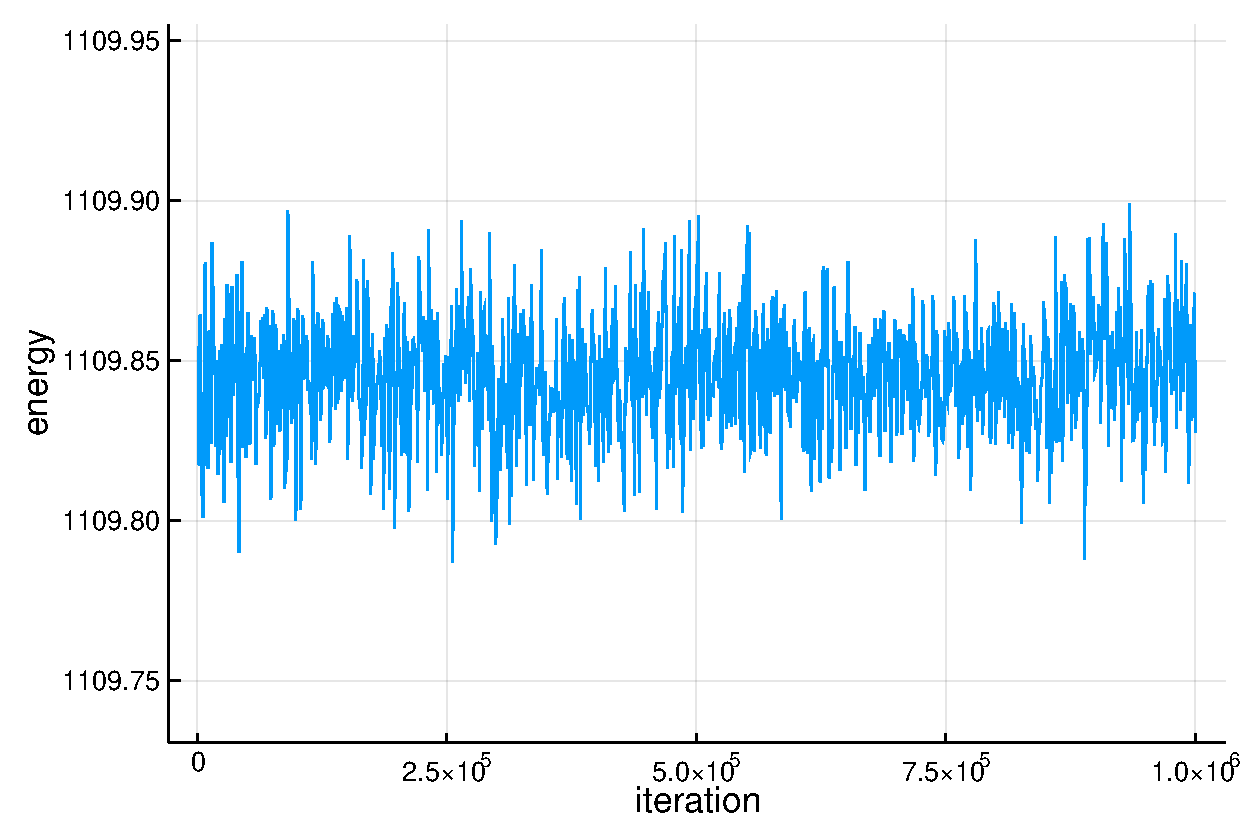
\includegraphics[scale=0.4]{plots/verlet_energy.pdf}
    \end{figure}

\end{frame}

\begin{frame}

    \frametitle{Schéma de Verlet}

    L'écart type de l'énergie croît comme $\Delta t^2$.

    \begin{figure}
        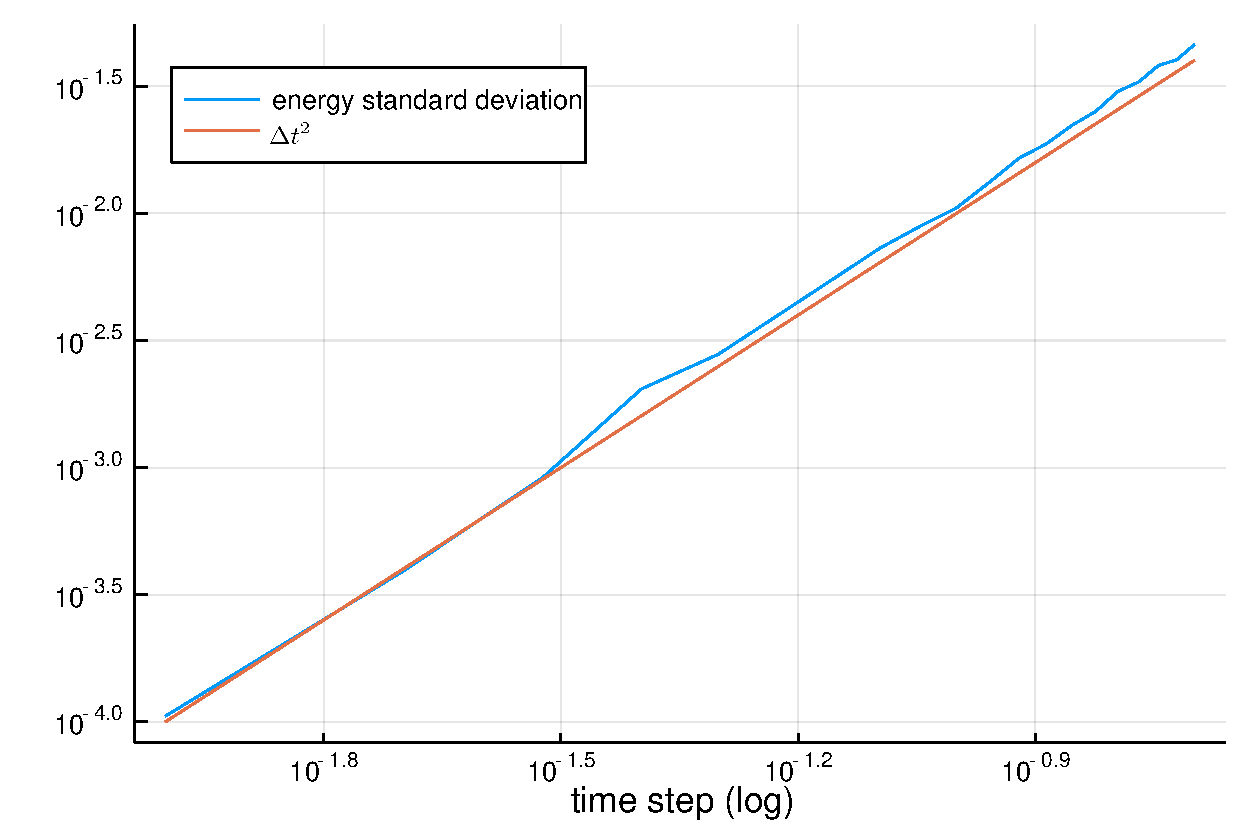
\includegraphics[scale=0.4]{plots/verlet_energy_spread.pdf}
    \end{figure}

\end{frame}

